\chapter*{Vorwort}

In den letzten Jahren wurden im Rahmen einer Reihe von Qualifizierungsarbeiten (Bachelor-, Master- und Projektarbeiten) im Bachelor-Studiengang \textit{Angewandte Mathematik} sowie im Master-Studiengang \textit{Optimierung \& Simulation} des Fachbereichs \textit{Ingenieurwissenschaften \& Mathematik} der Fachhochschule Bielefeld viele spezielle Untersuchungen an der Alltagsproblematik des jährlichen Laubharkens in Gärten oder Parks als ein spezifisch ausgeprägter Entsorgungsprozess vorgenommen. Hierbei wurden für unterschiedliche Fragestellungen spezifische Lösungsansätze entwickelt, die Eingang in ein Matlab-basiertes Programm (\glqq Laubharktool LHT\grqq{}) finden sollen. Mit diesem Tool sollen schließlich gezielte Effizienzanalysen vorgenommen werden können, um einem Anwender für analoge Problemausprägungen geeignete Lösungsverfahren anbieten zu können. \\
\\
In diesem Manuskript werden die theoretischen Grundlagen zusammenfasst, um die Implementierung der Lösungsansätze zu erleichtern, indem ein einheitlicher Formalismus vorgegeben wird und die Berechnungen der maßgeblichen Aufwände des gesamten Entsorgungsprozesses (Aufwände für Harken, Abtransportieren, unproduktive Wege) anhand von algorithmischen Beschreibungen angegeben werden. Zudem werden einige Harkstrategien vorgeschlagen (ebenfalls mit Pseudocodes).
\\ \\

\begin{center}
\begin{minipage}{\textwidth}
\centerline{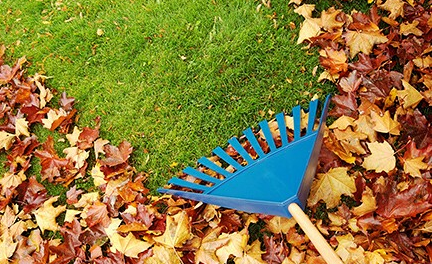
\includegraphics[angle=0,scale=4.0]{Figures/Laub/Titelfoto.png}}
\label{Titelfoto}
\end{minipage}
\end{center}